\part{Architectures des OS}

{
\setbeamertemplate{background canvas}{}
\begin{frame}[plain]
  \partpage
  \begin{textblock}{10}(6,11)
    %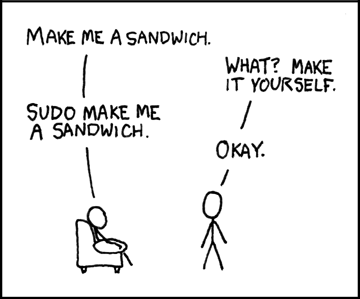
\includegraphics[height=30mm,width=30mm]{sandwich}
    \begin{quote}
      \rmfamily\textit\textbf\color{darkgray}{\large
        ``Why do programmers always mix up Halloween and Christmas?\\
        Because Oct 31 equals Dec 25.''}
      %\vskip3mm\hspace*\fill{\small--- William Shakespeare, Hamlet}
    \end{quote}
  \end{textblock}
\end{frame}
}

%\section{Les architectures standard}

\begin{frame}[fragile=singleslide]{Qu'est-ce qu'un noyau?}
  Un ensemble de services nécessitant une gestion centralisée
  \begin{itemize} 
  \item Ordonnanceur
  \item Gestionnaire de mémoire
  \item Drivers
  \item La gestion de  certains service nécessitant d'être centralisé:
    Réseau, les cache de disques, affichage vidéo
  \item  Les API  permettant  de communiquer  avec l'ordonnanceur,  le
    gestionnaire de mémoire (IPC, etc...) et les drivers
  \end{itemize} 
\end{frame} 

\begin{frame}[fragile=singleslide]{Qu'est-ce qu'un OS}
  Caractéristiques similaires au noyau (ordonnanceur, API, etc..) mais
  regroupe :
  \begin{itemize} 
  \item Les services fournis par le noyau
  \item Les  services fournis par des programmes  et des bibliothèques
    extérieures
  \end{itemize} 
\end{frame}

\begin{frame}{Composants de Linux}
  GNU/Linux est finalement un aggloméra:
  \\[2ex]
  \begin{center}
    \begin{tikzpicture}
      \filldraw[cbrown]
       (-0.05,0.95) -- +(9,0) -- +(9,1) -- +(8,1) -- +(8,2) -- +(7,2) -- +(7,3) 
       -- +(6,3) -- +(6,4) -- +(2,4) -- +(2,3) -- +(1,3) -- +(1,1) -- +(+0,1) -- cycle;
% node {Posix};
     \filldraw[ccyan]
       (7,5) -- +(1,0) -- +(1,-1) -- +(1.9,-1) -- +(1.9,0.9) -- +(0,0.9) -- cycle +(1,.5) node {App};
     \filldraw[ccyan]
       (1,5) rectangle +(1.9,0.9) +(1,.5) node {App};
     \filldraw[ccyan]
       (6,4) rectangle +(1.9,0.9) +(1,.5) node {App};
     \filldraw[cyellow]
       (4,4) rectangle +(1.9,0.9) +(1,.5) node {GNU App};
     \filldraw[cyellow]
       (2,4) rectangle +(1.9,0.9) +(1,.5) node {Bash};
     \filldraw[ccyan]
       (1.9,4) -- +(-1,0) -- +(-1,-2) -- +(-1.9,-2) -- +(-1.9,0.9) -- +(0,0.9) -- cycle +(-1,.5) node {App};
     %\filldraw[cyellow]
     %  (0,4) rectangle +(1.9,0.9) +(1,.5) node {App};
     \filldraw[cblue]
       (7,3) -- +(1,0) -- +(1,-1) -- +(1.9,-1) -- +(1.9,0.9) -- +(0,0.9) -- cycle +(1,.5) node {Lib};
     \filldraw[corange]
       (3,3) rectangle +(3.9,0.9) +(2,.5) node {GNU lib};
     \filldraw[corange]
       (1,2) -- +(6.9,0) -- +(6.9,0.9) -- +(1.9,0.9) -- +(1.9,1.9) -- +(0,1.9) -- cycle +(3.5,.5) node {GNU libc};
     \filldraw[cred]
       (0,1) rectangle +(8.9,0.9) +(4.5,.5) node {Noyau Linux};
     \filldraw[cgreen]
       (0,0) rectangle +(8.9,0.9) +(4.5,.5) node {Matériel};
    \end{tikzpicture}
  \end{center}
\end{frame}


\begin{frame}[fragile=singleslide]{Différents types d'architectures}
  On distingue alors:
  \begin{itemize} 
  \item  Les noyaux monolithiques.  Les drivers  et les  services sont
    gérés  dans un  même espace  mémoire.  Tous les  service du  noyau
    s'éxecute en superviseur.
  \item Les  micro-noyaux. Les drivers  et service s'éxecute  dans des
    contextes mémoire différents avec des accès restreints au système.
  \end{itemize} 
\end{frame}

\begin{frame}[fragile=singleslide]{Différents types d'architectures}
  Quelques remarques:
  \begin{itemize} 
  \item   Les  micro-noyaux   sont  plus   robustes  aux   erreurs  de
    développement des drivers
  \item Les micro-noyau possèdent peu d'appels systèmes
  \item  Les  noyau  monolithiques  sont  moins  lourds  en  terme  de
    transfert d'informations
  \item Les micro-noyau sont  plus complexe à architecturer. Tellement
    complexes  qu'il  n'existe pas  d'exemple  de micro-noyau  s'étant
    développé sur des architecture riches
  \end{itemize} 
\end{frame}


\begin{frame}[fragile=singleslide]{Différents types d'architectures}
  \begin{itemize} 
  \item XNU  (le noyau de MacOSX)  est un noyau  monolithique basé sur
    Mach 3 (monolithique aussi)
  \item Hurd, Beos et Mach 4, sont des micro-noyau (peu connus)
  \item Les  hyperviseurs tels  que Adeos ou  VMWare ESX  peuvent être
    apparenté à des micro-noyau (mais pas complètement)
  \item  Windows est  un  noyau hybride.  Windows exporte  suffisament
    d'API  pour  développer des  driver  à  l'extérieur  du noyau  (en
    partiulier les driver USB),  mais les drivers principaux sont dans
    le noyau (graphique, son, etc...)
  \item Linux est un noyau monolithique modulaire.
    \begin{itemize} 
    \item Débat Tanenbaum–Torvalds
    \item \url{http://groups.google.com/group/comp.os.minix/browse_thread/thread/c25870d7a41696d2}
    \item Modulaire depuis  la  version  2.6
    \end{itemize} 
  \item  Linux  permet  de  développer  certains types  de  drivers  à
    l'extérieur du noyau, mais ca  n'est pas son objectif et il montre
    rapidement ses limitations dans  le domaine (Serveur X, Fuse, UIO,
    CUPS, sane, libusb, etc...).
\end{itemize} 

\end{frame} 

% Environs 10 slides -> 30min

% Composition d'un OS multitache
%   Scheduler
%   Gestionnaire de mémoire
%   Des drivers
%   Une API et des services necessitant un "chef d'orchestre": IPC, réseaux, filesystèmes

% Petite partie, a placer avec la virtualisation?
% Noyau monolithique
%   .... mais modulaire
% Micronoyau
% Kernel Hybride
% Hyperviseurs
% Choix des méacanise de communication noyau/user et user/user
% 
% Divrsité de l'API
%   Nombre d'appels système: qqs uns comme Hurd, ou beaucoup comme Linux
%   API stable et definie (Linux) vs API movante (Windows)
%   "Schema de Linux" -> "Linux ne designe que le noyau, etc..."

%\section{La virtualisation}
